%% 美赛模板:正文部分

\documentclass[12pt]{article}  % 官方要求字号不小于 12 号,此处选择 12 号字体

% 本模板不需要填写年份,以当前电脑时间自动生成
% 请在以下的方括号中填写队伍控制号
\usepackage[2332102]{easymcm}  % 载入 EasyMCM 模板文件
\problem{Y}  % 请在此处填写题号
%\usepackage{mathptmx}  % 这是 Times 字体,中规中矩 
%\usepackage{mathpazo}  % 这是 COMAP 官方杂志采用的更好看的 Palatino 字体,可替代以上的 mathptmx 宏包
\usepackage{newtxtext}
\newcommand{\upcite}[1]{\textsuperscript{\textsuperscript{\cite{#1}}}} 
\title{Title}  % 标题

% 如需要修改题头(默认为 MCM/ICM),请使用以下命令(此处修改为 MCM)
\renewcommand{\contest}{MCM}

% 文档开始
\begin{document}

% 此处填写摘要内容
\begin{abstract}
    Sailboats fulfill diverse roles, fueling a thriving secondary market. Brokers, facing numerous complex factors, struggle to determine reasonable pricing. A tool to assist in comprehensive evaluations and rational pricing for used boats is urgently needed.
    
    This paper aims to construct a reliable model based on existing datasets, which can provide a reasonable explanation for the pricing of the second-hand sailboat market. It also analyzes the impact of different factors and indicators on prices. Finally, the model will be applied to the second-hand sailboat market in Hong Kong to provide a reasonable and accurate pricing rule.

    For Problem(a), \dots

    For Problem(b), \dots

    For Problem(c), \dots

    For Problem(d), \dots

    For Problem(e), \dots

    At the very last, we analyze the strengths and weaknesses of our model as well as its
sensitivity, whose results show that our model has high robustness, precision and accuracy.
After that, a report is attached.




    % 美赛论文中无需注明关键字。若您一定要使用,
    % 请将以下两行的注释号 '%' 去除,以使其生效
    \vspace{5pt}
    \textbf{Keywords}: heuristic hierarchical multiple regression, deep forest.

\end{abstract}

\maketitle  % 生成 Summary Sheet
\tableofcontents  % 生成目录


% 正文开始
\section{Introduction}
% 问题背景
\subsection{Background}
In our daily lives, sailboats are not only a means of transportation, but also serve as leisure and entertainment, and even for competitive sports. As a result, the growing demand for sailboats has given rise to a thriving boat market, which has gradually developed into a secondary market. In the secondary market, buyers and sellers usually trade through brokers, who play a crucial role in the transaction process.

For brokers, it is essential to be familiar with the used sailboat market, comprehensively consider various factors, and make reasonable pricing for the used sailboats in order to facilitate a successful transaction. However, the factors affecting the price of used sailboats are numerous and complex, with different brands, variants of boats, years, depreciation rates, as well as local consumption levels and geographical environments having significant impacts. The intertwined influences of these complex factors make it difficult to determine the pricing in the used sailboat market, and it is challenging to come up with a reasonable price that takes all factors into account.

Therefore, brokers urgently need a tool to assist them in making more reasonable and comprehensive evaluations of used sailboats, and to make the pricing in the used sailboat market more rational.
%问题重述
\subsection{Problem Restatement}
\textbf{Problem (a) :}
\begin{itemize}
    \item Develop a prediction model to explain the listing price of each of the sailboats in the provided spreadsheet.
    \item Discuss the precision of our estimate for each sailboat variant's price.
\end{itemize}

\textbf{Problem (b) :}
\begin{itemize}
    \item Determine whether region has an impact on the price of second-hand boats and explain the effect.
    \item Discuss whether any regional effect is consistent across all sailboat variants.
    \item Address the practical and statistical significance of any regional effects noted.
\end{itemize}

\textbf{Problem (c) :}
\begin{itemize}
    \item Based on the model, find out how it can be useful in the Hong Kong market.
    \item Choose one subset and model the regional effect of Hong Kong on each sailboat prices.
    \item Assess whether  the effect is the same for both catamarans and monohull sailboats.
\end{itemize}

\textbf{Problem (d) :}
\begin{itemize}
    \item Identify and discuss additional informative conclusions drawn from the data.
\end{itemize}

\textbf{Problem (e) :}
\begin{itemize}
    \item Create a one-to two-page report with well-chosen graphics to assist the Hong Kong sailboat broker to understand your findings.
\end{itemize}
%我们的工作
\subsection{Our work \& Model Overview}
\begin{figure}[htbp]
    \centering
    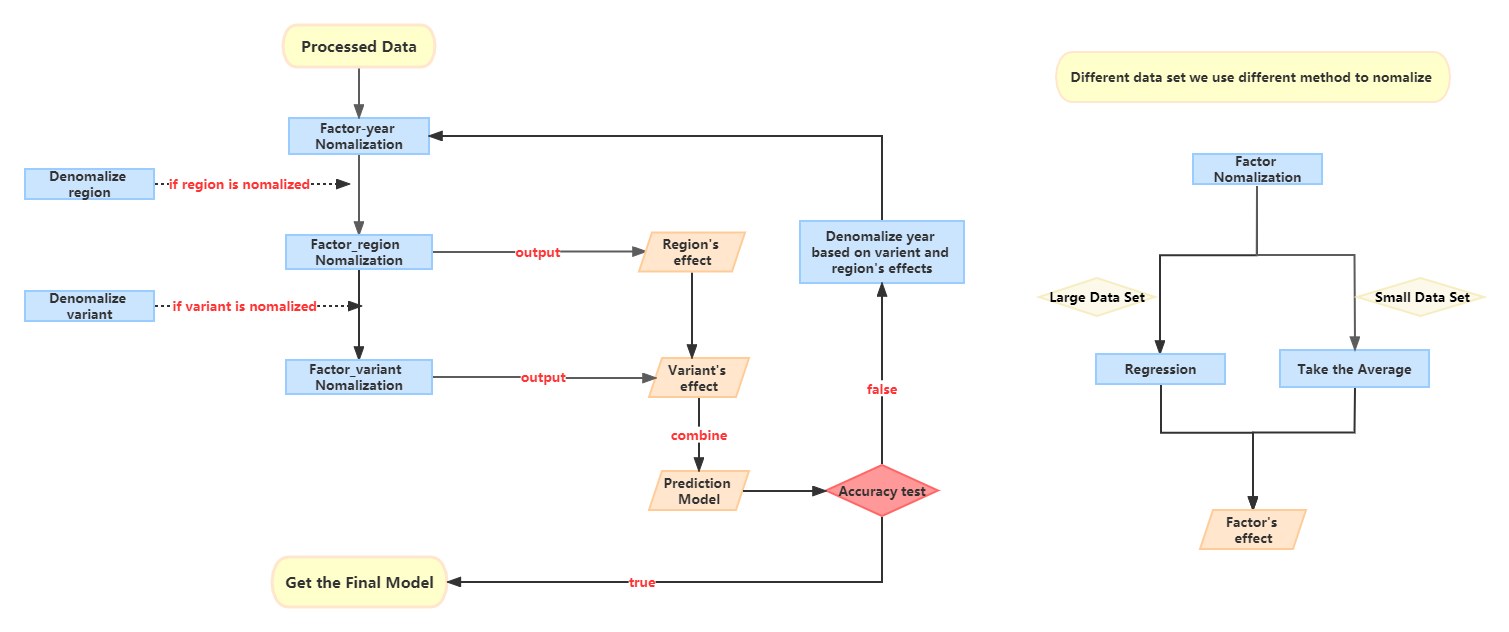
\includegraphics[width=1\textwidth]{Model.png}
    \caption{Model Framework}\label{fig:Model}
\end{figure}

We propose a model framework as shown in Figure \ref{fig:Model}, The model takes \texttt{Year}, \texttt{Region}, \texttt{Variant} as inputs, 
, \texttt{Price} as output, and performs a heuristic hierarchical multiple regression. 
Specifically, in each regression layer, one variable is denormalized, and the other two variables are normalized. 
The obtained \texttt{Price} at this time is used as the Effect of this variable. 
At the same time, the fitting result is used as the baseline for normalization in the next layer and is involved in the regression. 
This process is iterated continuously until the model trains a precise fitting effect.

It is worth noting that we use a heuristic approach for each normalization. 
For larger datasets, we perform regression, while for smaller datasets, we take their average. 
This method greatly improves the accuracy of the model predictions.
\section{Assumptions and Justififications}
% 问题假设
\subsection{Assumptions}
To simplify our problems, we make the following basic assumptions, each of which is
adequately justified.
\begin{itemize}
    \item The price of used sailboats is solely determined by the factors in the dataset.
    \item The factors in the dataset are independent and unrelated.
    \item The data in the dataset are all real, reasonable, and follow a certain pattern.
    \item The pricing required by a broker should be reasonable and in accordance with market rules, rather than false pricing.
\end{itemize}
%符号含义
\subsection{Notations}
\ 
% 三线表示例
\begin{table}[!htbp]
\begin{center}
\begin{tabular}{cl}
	\toprule
	\multicolumn{1}{m{3cm}}{\centering Symbol}
	&\multicolumn{1}{m{8cm}}{\centering Definition}\\
	\midrule
	$A$&the first one\\
	$b$&the second one\\
	$\alpha$ &the last one\\
	\bottomrule
\end{tabular}
\end{center}
\end{table}
\section{Data Exploration}
\begin{figure}[htbp]
    \centering
    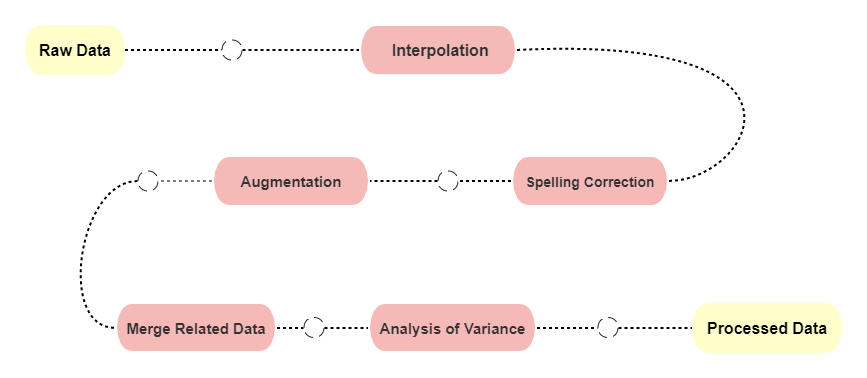
\includegraphics[width=1\textwidth]{Data.png}
    \caption{Data Exploration}\label{fig:Data}
\end{figure}

\subsection{Data Cleaning}
First of all, we turn the \textbf{\texttt{xlsx}} format data sheet into \textbf{\texttt{csv}} format. 
The conversion causes some minor errors like extra spaces and unexcepted characters which can be easily filtered out by text editor and python string operating functions like \textbf{\texttt{strip()}} or so.

Secondly, we use \textbf{Linear interpolation} to fill in the missing data and then apply \textbf{Adaptive Density-Based Clustering} for spell correction,
resulting in a more complete and accurate dataset than the original.

Further more, we merge \textbf{Make} and \textbf{Variant} into a single feature, which we refer to as \textbf{Variant}.

Finally, we merge the corrected dataset with the accurate one after making necessary modifications.
\begin{figure}[htbp]
    \centering
    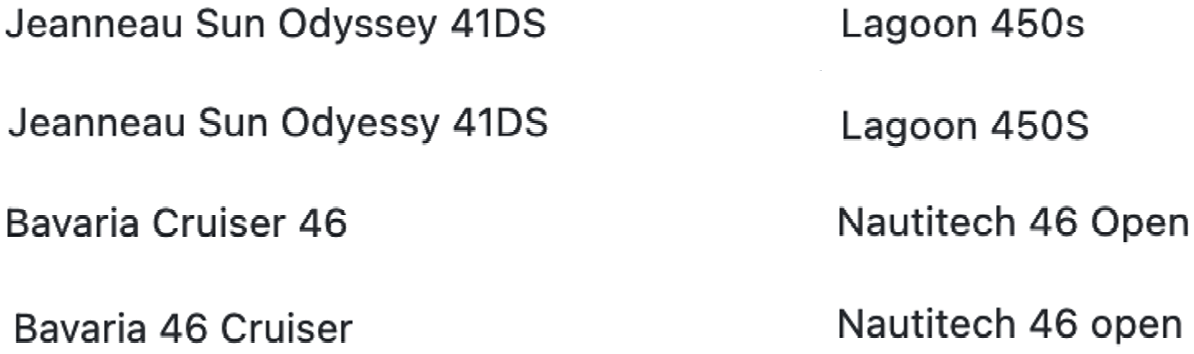
\includegraphics[width=0.7\textwidth]{error_data.png}
    \caption{Examples of error data}\label{fig:error_data}
\end{figure}

\subsection{Data Analysis}

\subsection{Data Augmentation}
We collect and organize more additional features of a given sailboat(such as \textbf{beam}, \textbf{draft}, \textbf{displacement}, \textbf{cabins}, etc.),
and the \textbf{2020 per capita GDP data} of the relevant regions, 
greatly enriching the diversity of the data and expanding the dataset size. 
These efforts lay a solid foundation for subsequent modeling.

\section{The Prediction Model of Used Sailboat Prices}
\subsection{The Establishment of The Model}

\subsection{Model Validation}
\subsection{Model Accuracy Analysis}


\section{Regional Effect Analysis}

\section{The applicability of The Prediction Model in Hong Kong}

\section{Extended Inferences or Conclusion}

\section{Further Improvements}

\section{Strengths and Weaknesses}
\subsection{Strengths}
\begin{itemize}
    \item First one...
    \item Second one ...
\end{itemize}

\subsection{Weaknesses}
\begin{itemize}
    \item Only one ...
 \end{itemize}

\section{Conclusion}


% 以下为信件/备忘录部分,不需要可自行去掉
% 如有需要可将整个 letter 环境移动到文章开头或中间
% 请在第二个花括号内填写标题,如「信件」(Letter)或「备忘录」(Memorandum)
\begin{letter}{Report}
\noindent\rule[0.25\baselineskip]{\textwidth}{2pt} 
\begin{flushleft}  % 左对齐环境,无首行缩进
\textbf{To:} Heishan Yan\\
\textbf{From:} Team 1234567\\
\textbf{Date:} October 1st, 2019\\
\textbf{Subject:} A better choice than MS Word: \LaTeX
\end{flushleft}

In the memo, we want to introduce you an alternate typesetting program to the prevailing MS Word: \textbf{\LaTeX}. In fact, the history of \LaTeX\ is even longer than that of MS Word. In 1970s, the famous computer scientist Donald Knuth first came out with a typesetting program, which named \TeX\ \ldots

Firstly, \ldots

Secondly, \ldots

Lastly, \ldots

According to all those mentioned above, it is really worth to have a try on \LaTeX! 
\end{letter}


% 参考文献,此处以 MLA 引用格式为例
\begin{thebibliography}{99}
\bibitem{1} Einstein, A., Podolsky, B., \& Rosen, N. (1935). Can quantum-mechanical description of physical reality be considered complete?. \emph{Physical review}, 47(10), 777.
\bibitem{2} \emph{A simple, easy \LaTeX\ template for MCM/ICM: EasyMCM}. (2018). Retrieved December 1, 2019, from\url{https://www.cnblogs.com/xjtu-blacksmith/p/easymcm.html}
\end{thebibliography}


% 以下为附录内容
% 如您的论文中不需要附录,请自行删除
\begin{subappendices}  % 附录环境

\section{Appendix A: Further on \LaTeX}
To clarify the importance of using \LaTeX\ in MCM or ICM, several points need to be covered, which are \ldots

To be more specific, \ldots

All in all, \ldots

Anyway, nobody \textbf{really} needs such appendix \ldots

\section{Appendix B: Program Codes}
Here are the program codes we used in our research.

% 代码环境示例三则
% 如您的论文不需要展示代码,请删除
% 更多用法,请参考 listings 宏包文档

% Python 代码示例
\begin{lstlisting}[language=Python, name={test.py}]
# Python code example
for i in range(10):
    print('Hello, world!')
\end{lstlisting}

% MATLAB 代码示例
\begin{lstlisting}[language=MATLAB, name={test.m}]
% MATLAB code example
for i = 1:10
    disp("hello, world!");
end
\end{lstlisting}

% C++ 代码示例
\begin{lstlisting}[language=C++, name={test.cpp}]
// C++ code example
#include <iostream>
using namespace std;

int main() {
    for (int i = 0; i < 10; i++)
        cout << "hello, world" << endl;
    return 0;
}
\end{lstlisting}

\end{subappendices}  % 附录内容结束

\end{document}  % 结束
